\hypertarget{create-a-usb-stick-with-ubuntu-from-osx}{%
\section{Create a USB stick with Ubuntu from
OSX}\label{create-a-usb-stick-with-ubuntu-from-osx}}

The original Web page for this method is available at

\begin{itemize}
\tightlist
\item
  \url{https://help.ubuntu.com/community/How\%20to\%20install\%20Ubuntu\%20on\%20MacBook\%20using\%20USB\%20Stick}
\end{itemize}

We have copied some of the information from this Web page but made
enhancements to it. Our goal is to create a USB stick that has either
Ubuntu 16.04.03 or ubuntu 17.10.1 on it.

This can be achieved while visiting the URL

\begin{itemize}
\tightlist
\item
  \url{https://www.ubuntu.com/download/desktop}
\end{itemize}

First we assume that you downloaded to iso from ubuntu to a folder
called \emph{iso}. Next we open a terminal and cd into the folder
\emph{iso}. Now we need to convert the is to an image file. This is done
as follows and you need to execute the command for the version of ubuntu
you like to use.

Your folde will look something like this

\begin{verbatim}
ls -1

    ubuntu-16.04.3-desktop-amd64.iso
    ubuntu-17.10.1-desktop-amd64.iso
\end{verbatim}

For 17.10.1 you will need to generate an image with the following
command

\begin{verbatim}
hdiutil convert ubuntu-17.10.1-desktop-amd64.iso -format UDRW -o ubuntu-17.10.1-desktop-amd64.img
\end{verbatim}

For 16.04.3 you will need to generate an image with the following
command

\begin{verbatim}
hdiutil convert ubuntu-16.04.3-desktop-amd64.iso -format UDRW -o ubuntu-16.04.3-desktop-amd64.img
\end{verbatim}

OSX will append a .dmg behind the name. When considering the OS and you
only want to use one, we recommend that you use the latest OS. Please
let us know if we need to update the verion numbers. Check with the
ubuntu Web page.

At this time do not plug in your usb stick. Just issue the command

\begin{verbatim}
diskutil list
\end{verbatim}

Observe the output. Now plug in the USB stick. Wait till the USB stick
registers in the Finder. If this does not work find a new USB stick or
format it. Execute the command

\begin{verbatim}
diskutil list
\end{verbatim}

and observer the output again. Another devce will register and you will
see something like

\begin{verbatim}
/dev/disk2 (external, physical):
#:     TYPE NAME               SIZE       IDENTIFIER
0:     FDisk_partition_scheme *8.2 GB     disk2
1:     DOS_FAT_32 NO NAME      8.2 GB     disk2s1
\end{verbatim}

Please note in this example the device path and number is recognized as

\begin{verbatim}
/dev/disk2
\end{verbatim}

It also says external, which is a good sign as the USB stick is
external. Next, we need to unmoundt the device with

\begin{verbatim}
diskutil unmountDisk /dev/diskN
\end{verbatim}

where you replace the number N with the disk number that you found for
the device. In our example it would be 2. If you see the error ``Unmount
of diskN failed: at least one volume could not be unmounted'', start
Disk Utility.app and unmount the volume (don't eject). If it was
successful, you will see

\begin{verbatim}
Unmount of all volumes on disk2 was successful
\end{verbatim}

The next step is dangerous and you need to make sure you follow it. So
please do not copy and paste, but read first, reflect and only if you
understand it execute it. We know we say this all the time, but better
saying it again instead of you destryoing your system. This command also
requires sudo access so you will either have to be in the sudo group, or
use

\begin{verbatim}
su <your administrator name>
\end{verbatim}

login and than execute the command under root.

\begin{verbatim}
sudo dd if=ubuntu-17.10.1-desktop-amd64.img.dmg of=/dev/diskN bs=1m
\end{verbatim}

(Not tested: Using /dev/rdisk instead of /dev/disk may be faster
according to the ubuntu documentation)

Ubuntu's Web page also gives the following tips:

\begin{itemize}
\tightlist
\item
  ``If you see the error dd: Invalid number `1m', you are using GNU dd.
  Use the same command but replace bs=1m with bs=1M.''
\item
  ``If you see the error dd: /dev/diskN: Resource busy, make sure the
  disk is not in use. Start Disk Utility.app and unmount the volume
  (don't eject).''
\end{itemize}

You will see an error window popping up telling you: \textbf{The disk
inserted was not readbale by this compute}. Please, leave the window as
is and instead type in on the terminal.

\begin{verbatim}
diskutil eject /dev/diskN
\end{verbatim}

Now remove the flash drive, and press in the error window
\textbf{Ignore}\\
Now you have a falsh drive with ubuntu installed and you can boot from
it. To do so, please

\textbf{restart your Mac and press option key}

while the Mac is restarting to choose the USB-Stick

You will need a plug for USB keyboard, USB mouse, and netwwork cable.

There are some issue from this point on.

\begin{verbatim}
sudo apt-get update
\end{verbatim}

Add univers to the window for application updates

see https://help.ubuntu.com/community/Repositories/Ubuntu

\begin{verbatim}
sudo apt-get install vnc4server
\end{verbatim}

Start the server and set up a password

\begin{verbatim}
vncserver
\end{verbatim}

\textbf{WARNING: UNTESTED FOR NOW}

\hypertarget{ubuntu-on-a-usb-stick-for-osx}{%
\section{Ubuntu on a USB stick for
OSX}\label{ubuntu-on-a-usb-stick-for-osx}}

The material in thi section was copied from

\begin{itemize}
\tightlist
\item
  https://tutorials.ubuntu.com/tutorial/tutorial-create-a-usb-stick-on-macos
\end{itemize}

\hypertarget{requirements}{%
\subsection{Requirements}\label{requirements}}

You will need:

\begin{itemize}
\tightlist
\item
  A 2GB or larger USB stick/flash drive
\item
  An Apple computer or laptop running macOS
\item
  An Ubuntu ISO file. See Get Ubuntu for download links
  https://www.ubuntu.com/download
\end{itemize}

\hypertarget{install-etcher}{%
\subsection{Install Etcher}\label{install-etcher}}

To write the ISO file to the USB stick, we're going to use a free and
open source application called Etcher. After downloading this and
clicking to mount the package, Etcher can either be run in-place or
dragged into your Applications folder.

\begin{itemize}
\tightlist
\item
  https://etcher.io/
\end{itemize}

By default, recent versions of macOS block the running of applications
from unidentified developers. To side-step this issue, enable `App Store
and identified developers' in the `Security \& Privacy' pane of System
Preferences. If you are still warned against running the application,
click `Open Anyway' in the same pane.

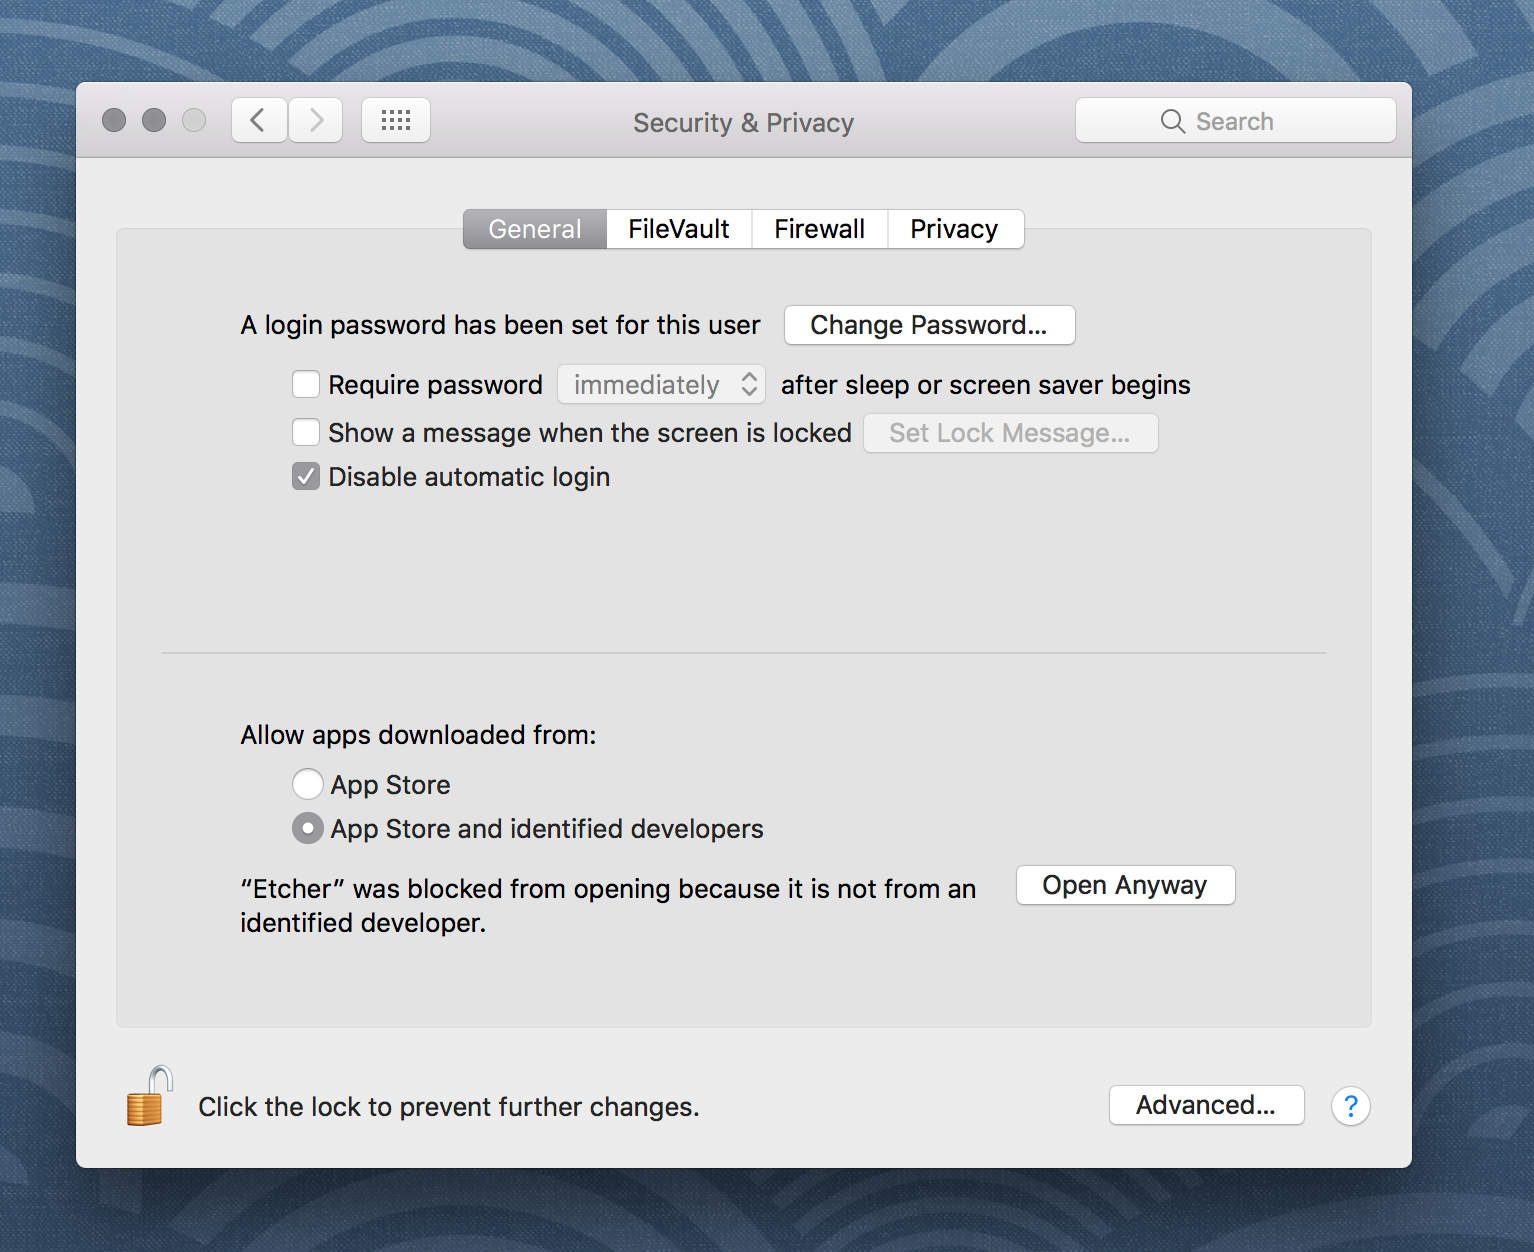
\includegraphics{https://tutorials.ubuntu.com/es6-bundled/src/codelabs/tutorial-create-a-usb-stick-on-macos/img/49647529d8a4f32b.png}

\hypertarget{prepare-the-usb-stick}{%
\subsection{Prepare the USB stick}\label{prepare-the-usb-stick}}

\textbf{Warning: Disk Utility needs to be used with caution as selecting
the wrong device or partition can result in data loss.}

\begin{itemize}
\tightlist
\item
  Launch Disk Utility from Applications\textgreater{}Utilities or
  Spotlight search
\item
  Insert your USB stick and observe the new device added to Disk Utility
\item
  Select the USB stick device and select Erase from the tool bar (or
  right-click menu)
\item
  Set the format to MS-DOS (FAT) and the scheme to GUID Partition Map
  Check you've chosen the correct device and click Erase
\end{itemize}

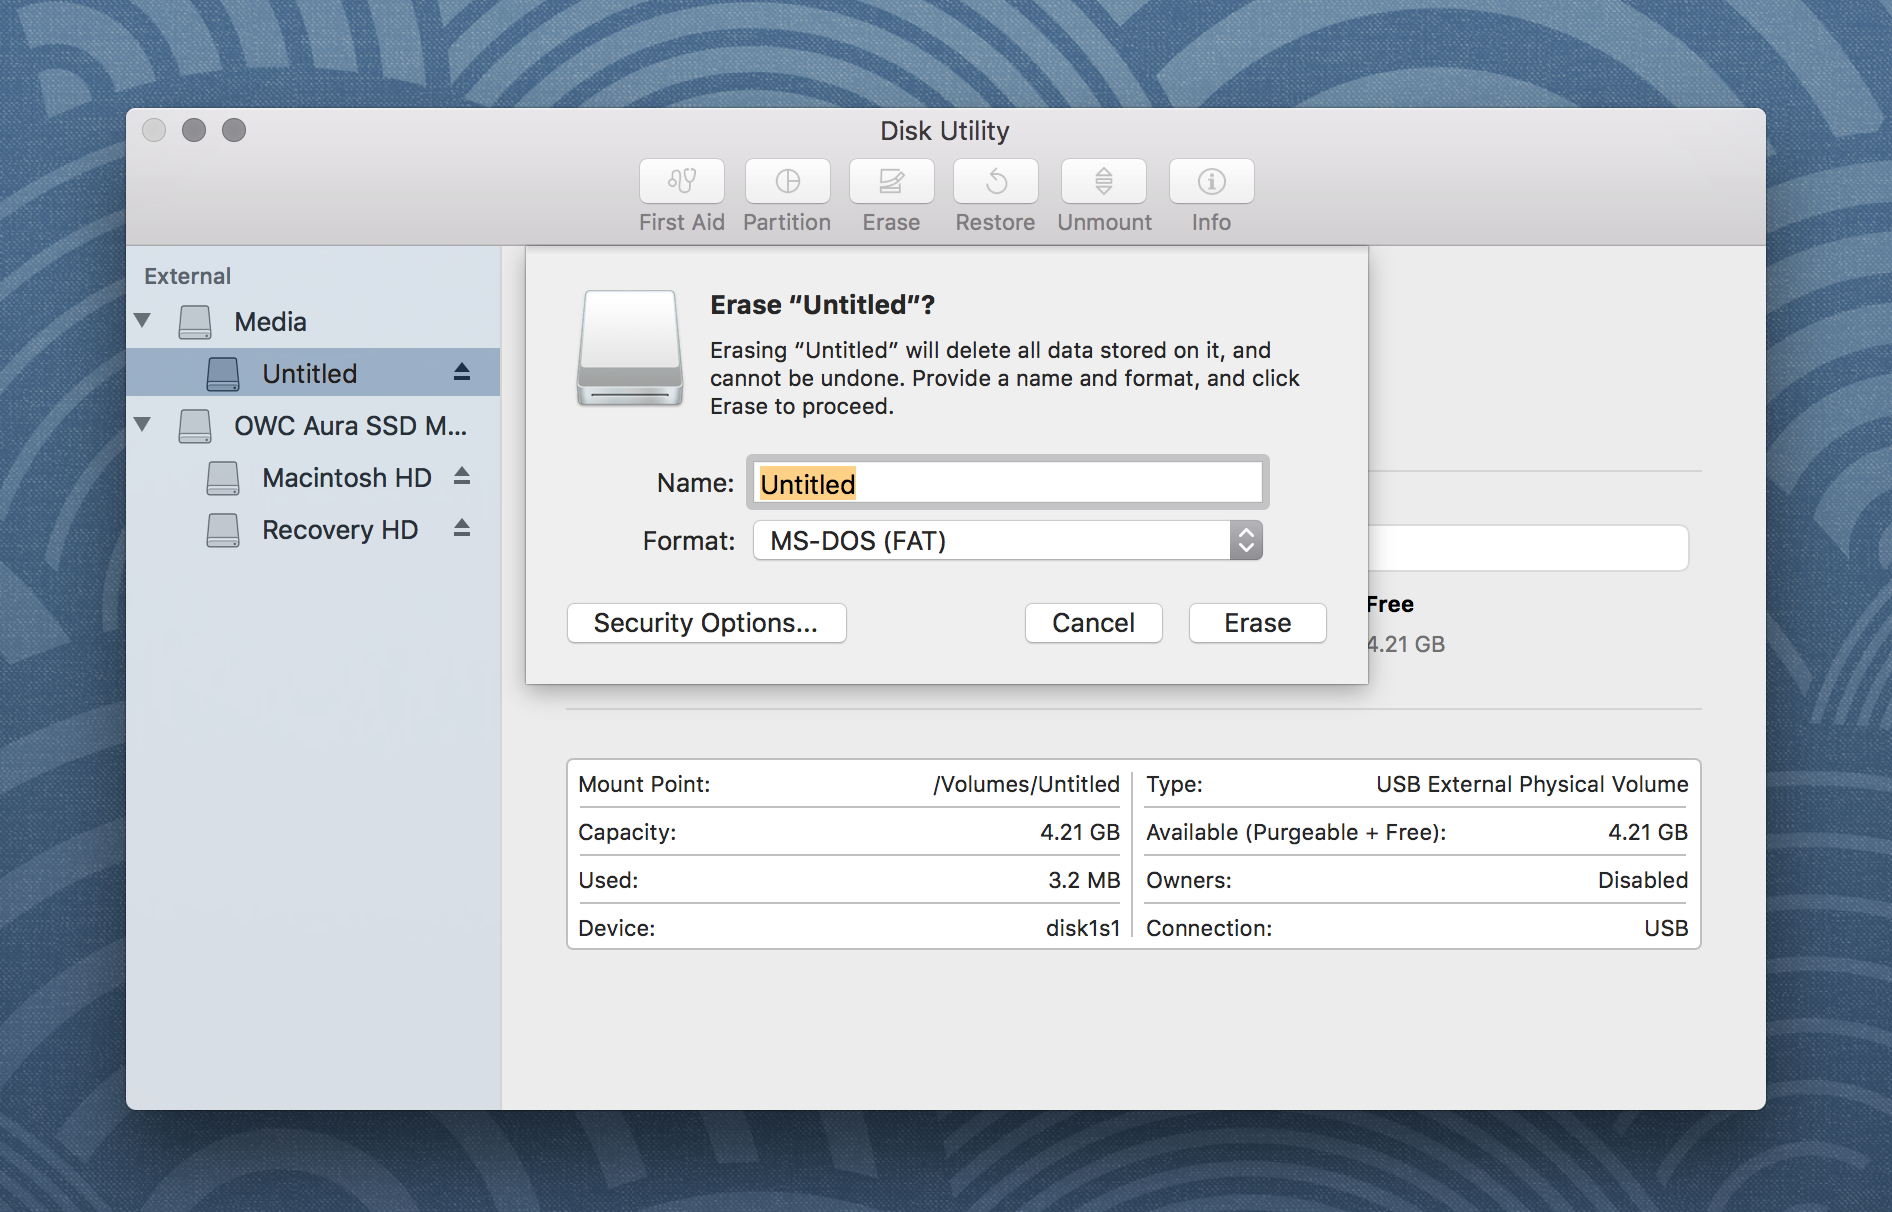
\includegraphics{https://tutorials.ubuntu.com/es6-bundled/src/codelabs/tutorial-create-a-usb-stick-on-macos/img/14c3877ad1c43497.png}

\hypertarget{etcher-configuration}{%
\subsection{Etcher configuration}\label{etcher-configuration}}

Etcher will configure and write to your USB device in three stages, each
of which needs to be selected in turn:

\begin{itemize}
\tightlist
\item
  Select image will open a file requester from which should navigate to
  and select the ISO file downloaded previously. By default, the ISO
  file will be in your Downloads folder.
\item
  Select drive, replaced by the name of your USB device if one is
  already attached, lets you select your target device. You will be
  warned if the storage space is too small for your selected ISO.
\item
  Flash! will activate when both the image and the drive have been
  selected. As with Disk Utility, Etcher needs low-level access to your
  storage hardware and will ask for your password after selection.
\end{itemize}

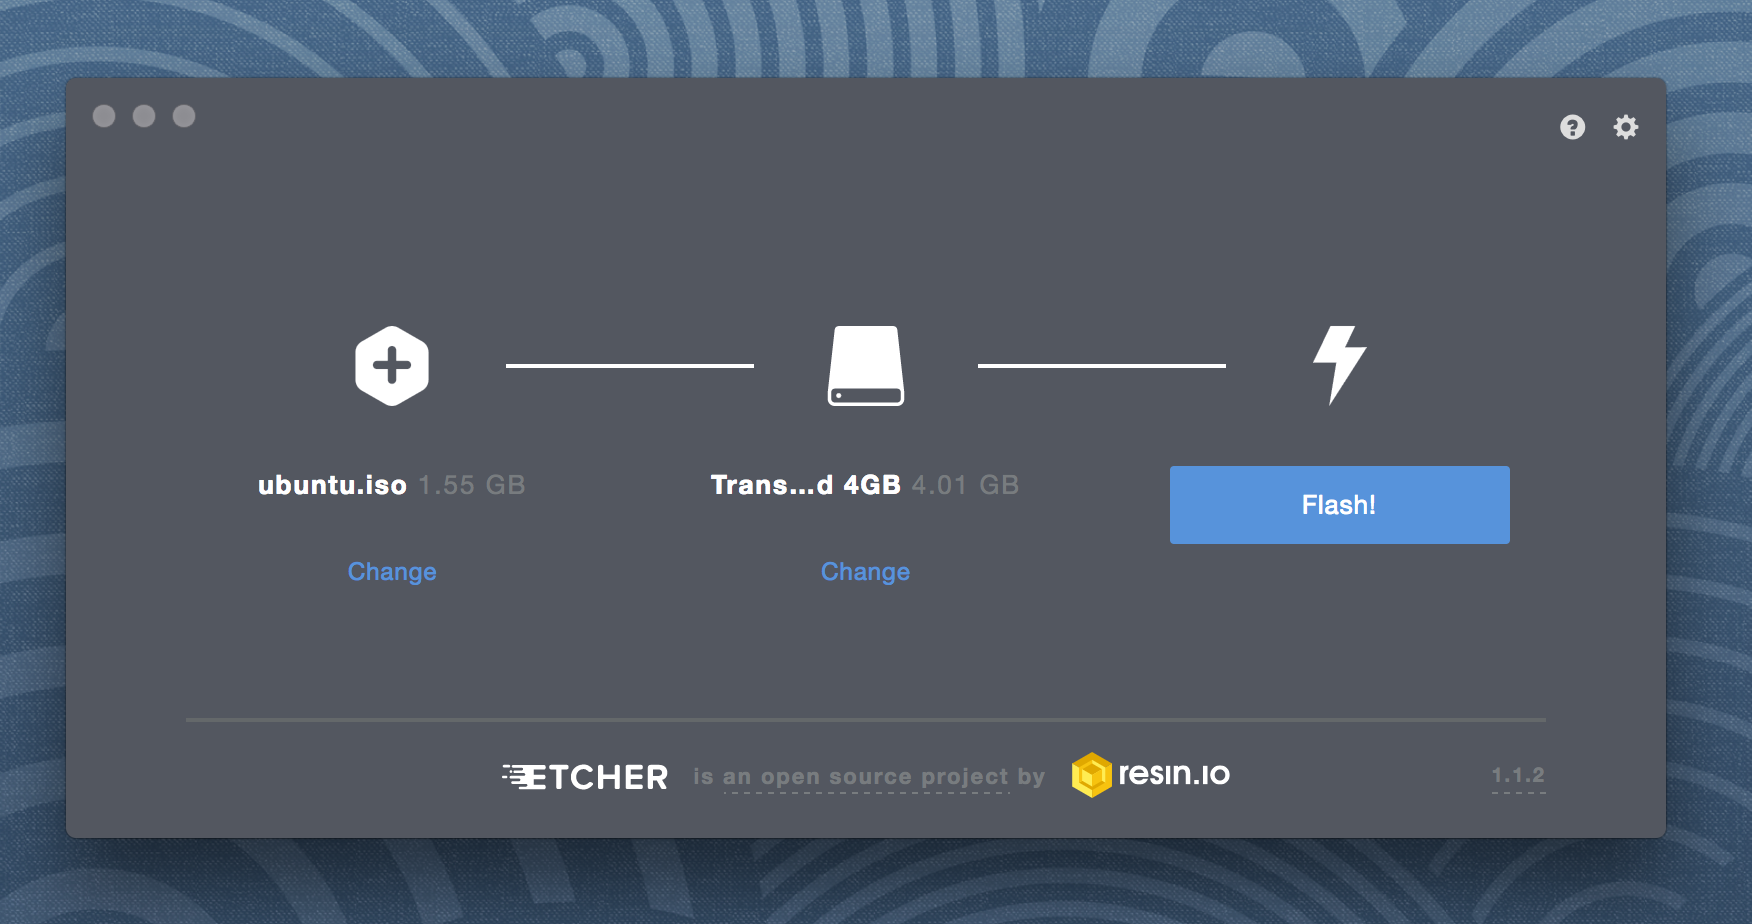
\includegraphics{https://tutorials.ubuntu.com/es6-bundled/src/codelabs/tutorial-create-a-usb-stick-on-macos/img/3bb88ce0bc88abb3.png}

\hypertarget{write-to-the-usb-stick}{%
\section{Write to the USB stick}\label{write-to-the-usb-stick}}

Write to device

After entering your password, Etcher will start writing the ISO file to
your USB device.

The Flash stage of the process will show progress, writing speed and an
estimated duration until completion. This will be followed by a
validation stage that will ensure the contents of the USB device are
identical to the source image.

When everything has finished, Etcher will declare the process a success.

Congratulations! You now have Ubuntu on a USB stick, bootable and ready
to go.

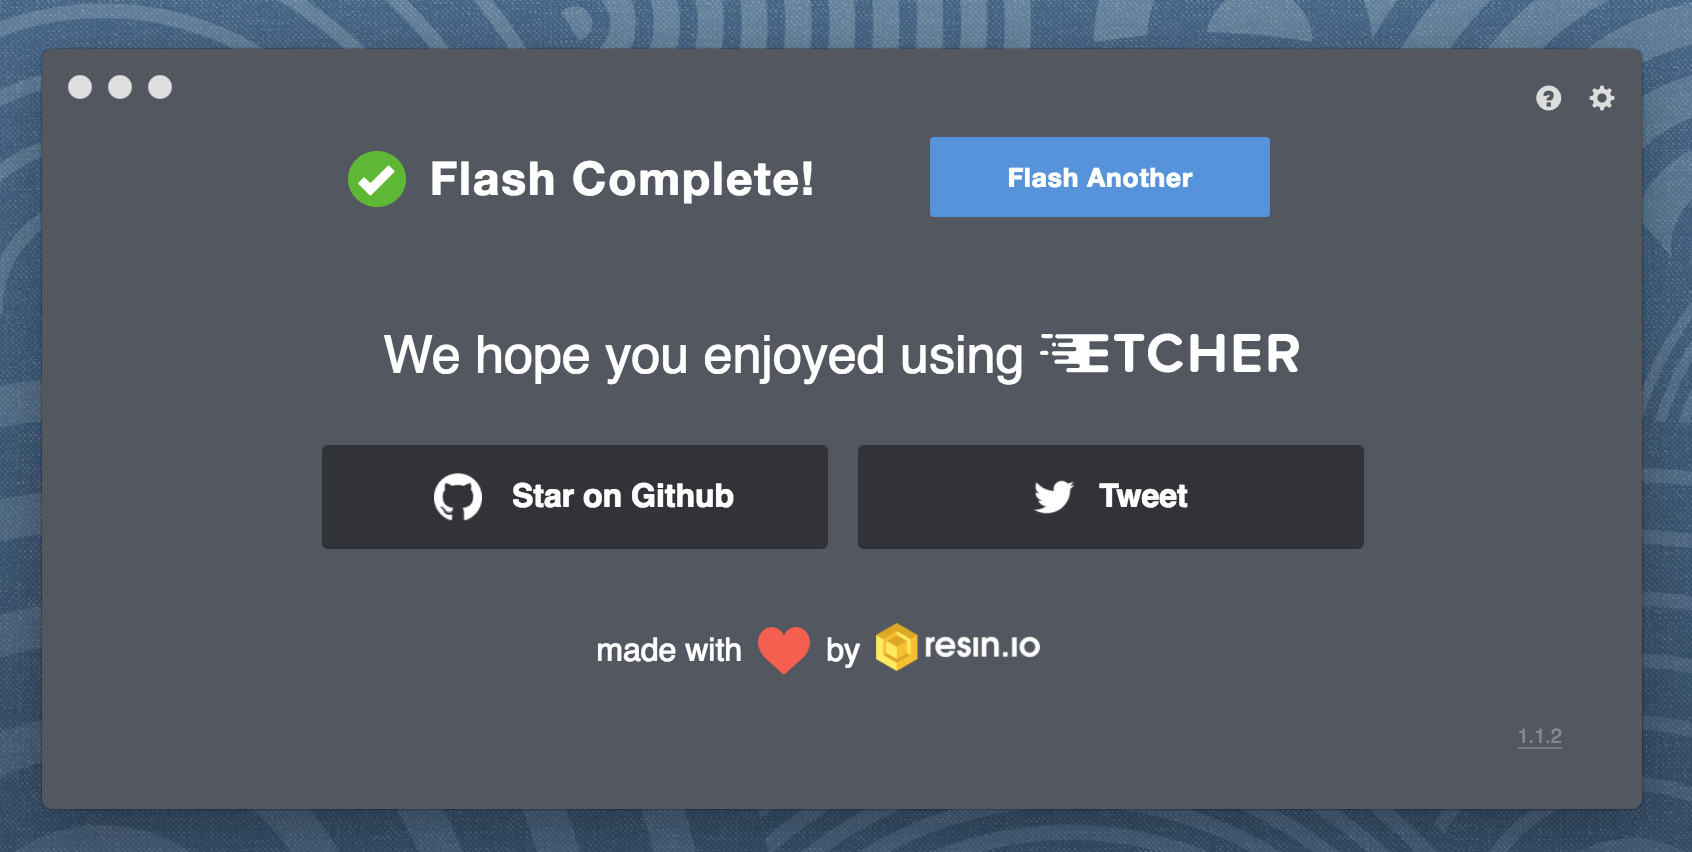
\includegraphics{https://tutorials.ubuntu.com/es6-bundled/src/codelabs/tutorial-create-a-usb-stick-on-macos/img/4207a01ff6afea52.png}

\textbf{Warning: After the write process has completed, macOS may inform
you that `The disk you inserted was not readable by this computer'.
Don't select Initialise. Instead, select Eject and remove the USB
device.}

\hypertarget{boot-from-the-usb-stick}{%
\subsection{Boot from the USB Stick}\label{boot-from-the-usb-stick}}

oot your Mac

If you want to use your USB stick with an Apple Mac, you will need to
restart or power-on the Mac with the USB stick inserted while the
Option/alt(⌥) key is pressed.

This will launch Apple's `Startup Manager' which shows bootable devices
connected to the machine. Your USB stick should appear as gold/yellow
and labelled `EFI Boot'. Selecting this will lead you to the standard
Ubuntu boot menu.

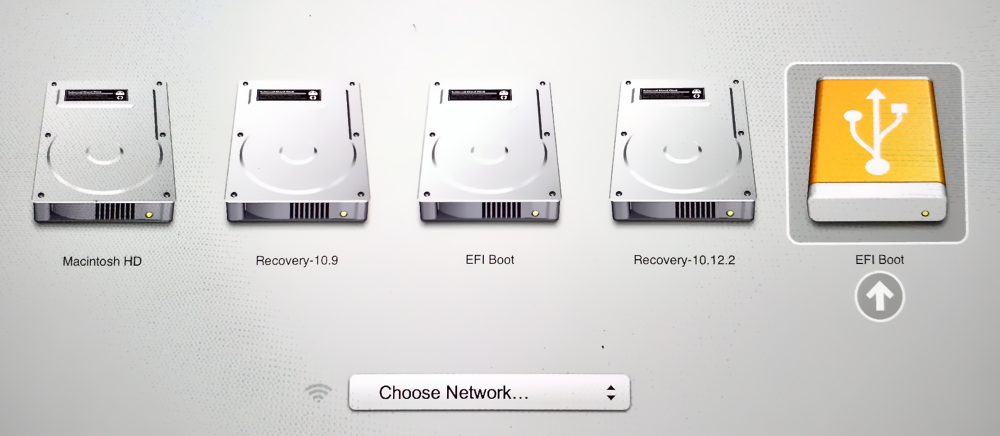
\includegraphics{https://tutorials.ubuntu.com/es6-bundled/src/codelabs/tutorial-create-a-usb-stick-on-macos/img/ba4c21e1ca753cf.png}

If you want to install Ubuntu, follow our install Ubuntu desktop
tutorial.

\begin{itemize}
\tightlist
\item
  https://tutorials.ubuntu.com/tutorial/tutorial-install-ubuntu-desktop\#0
\end{itemize}
